\ProvidesFile{ch-light-curve-inversion.tex}[Light Curve Shape Inversion]
\graphicspath{{/Users/liamrobinson/Documents/msthesis/static_images/aas_2022_figs}}
\chapter{Light Curve Shape Inversion}

\section{Nature of The Problem}

The problem of light curve shape inversion is plagued by different types of ambiguities. In order to understand the later inversion methods, it is important to understand the characteristics of each ambiguity.

\subsection{True Ambiguities}

A true ambiguity exists in the shape inversion problem due to the interplay between the coefficients of reflection of the object's surfaces and their areas. Often, these factors are considered together as the \textit{albedo-area}. For a given shape, there exist an infinite family of geometrically similar shapes which possess the same albedo area with face areas scaled by a nonzero scalar $c$ and coefficients of reflection scaled by $a^{-1}$, constrained such that the scaled face albedo cannot violate energy conservation \cite{fan2020thesis}. This family produces the same light curve in the same observation conditions, and is thus no decision can be made about the object's true scale within this family without additional information. In practice, knowledge of standard properties of common materials may be used to further constrain the scale of the object, but nonzero true ambiguities always remain.

\subsection{Convex Observability Ambiguities}

Depending on the object attitude profile and the geometry of the observer and the Sun, some faces of the object may never be illuminated and observed at the same time. In such cases, both the area and normal vector of the face are unobservable. The geometry of a convex object in these unobserved areas is unconstrained by the light curve alone.

\subsection{Nonconvex Shape Ambiguities}

The influence of concavities are only observable in the light curve due to the variability of self-shadowing. If viewed at a constant phase angle of $\phi = 0^\circ$ between the Sun and observer vectors, no self-shadowing can occur and the resulting light curve will be well-fit by a convex estimate. Similarly, a concavity that is never illuminated or is never able to be observed while illuminated is unobservable as its self-shadowing effects are not present in the observed light curve. 

If a concave feature does contribute to the light curve while self-shadowing is occurring, new ambiguities are introduced. A single concave feature can be broken up into multiple smaller concavities with the same interior geometry and proportionally smaller face areas. Similarly, other concavity geometries may produce the same aggregate effect on the light curve.

\subsection{Bayesian Inversion}

Bayes' theorem is stated \cite{mahler2014}:

\begin{equation}
  P(A \vert B) = \frac{P(B \vert A)P(A)}{P(B)},
\end{equation}

where $A$ and $B$ are two events and $P(B) \neq 0$. In the context of shape inversion, we seek to find the shape $A$ that best explains the light curve $B$. To evaluate the probability of a given shape mesh estimate $\mathcal{M}_i$ based on light curve data $I_{1:i}$, the quantities $P(\mathcal{M}_i)$ and $P(I_{1:i})$ are required. The probability of a given mesh estimate $P(\mathcal{M}_i)$ is difficult to evaluate, as it is not clear how to define a prior distribution over the space of all possible meshes. As a result, it is impractical to perform a full Bayesian update on a given shape estimate.

\section{Direct Convex Shape Inversion}

Traditionally, direct light curve inversion involves two distinct optimization problems: a linear least squares problem to optimize normal vectors and areas to match the measured light curve, and a second optimization to produce accurate vertex positions and face adjacency information \cite{fan2020thesis, kaasalainen2000, kaas2001shape, cabrera2021}. The first problem is data-driven and linear, using the observations to estimate a plausible EGI. The second problem is highly nonlinear but convex and requires significant tuning for robust convergence \cite{fan2019}. The full convex inversion process presented in this work is outlined:

\begin{outline}[enumerate]
  \1 Area and normal vector optimization
    \2 Initial normal vector sampling
    \2 Initial face area optimization
    \2 Normal vector resampling
    \2 Face area reoptimization
    \2 Face merging
  \1 Object reconstruction
    \2 Face support optimization
    \2 Dual transform yielding final vertex locations
    \2 Convex hull yielding final face adjacency relationships
\end{outline}

\subsection{The Extended Gaussian Image} \label{sec:egi_definition}

In the continuous case, the Gaussian Image associates each point on the surface of a shape with a outward-pointing normal vector direction on the unit sphere $\mathbb{S}^2$ \cite{horn1984}. The determinant of the Jacobian of this forward mapping yields the Gaussian curvature $\kappa(u,v)$ of the surface at each surface point --- expressing how rapidly local normal vectors change direction \cite{horn1984}. The continuous \textit{Extended} Gaussian Image (EGI) $E(\theta, \phi)$ is a function on the unit sphere parameterized by an azimuth $\theta$ and elevation $\phi$ which sums the inverse Gaussian curvature for all points $(u_i, v_i)$ on the surface of the object with a normal pointing towards $(\theta, \phi)$ \cite{horn1984}:

\begin{equation} \label{eq:egi_deg}
  E(\theta, \phi) = \sum_i{\frac{1}{\| \kappa(u_i, v_i) \|}}.
\end{equation}

By Eq \ref{eq:egi_deg}, flat areas of the object are mapped to point masses in the EGI, motivating a simpler definition of the EGI for discrete surfaces. The discrete EGI $\vec{E} \in \mathbb{R}^{m \times 3}$ is composed of $m$ unit vectors $\hat{n}$ each scaled by a nonnegative areea $a \in \mathbb{R}$, where $a_i \geq 0 \forall i$ \cite{little1983}.

\begin{equation}
  \vec{E}_i = a_i \hat{n}_i
\end{equation}

In the context of shape inversion, the $m$ vectors $\hat{n}$ should be a relatively uniform tessellation of the unit sphere. A convex polytope can be uniquely represented by an EGI of facet normal vectors scaled by each facet's area. The set of normal vectors in an EGI is denoted $\mathcal{N}$ with the set of areas denoted $\mathcal{A}$. The vector of facet areas is denoted $\vec{a} \in \mathbb{R}^{m \times 1}$. The norm of the EGI is notated $\| \vec{E} \| = \vec{a}$ with the `size' of the EGI $\|\vec{E}\| = m$.

The solution to the Minkowski problem proves the existence and uniqueness of a convex polytope for any EGI satisfying the closure condition \cite{minkowski1909}:

\begin{equation} \label{eq:egi_closure}
  \sum_{i=1}^m a_i \hat{n}_i = [0, 0, 0].
\end{equation}

Equivalently, an EGI uniquely represents a closed, convex polyhedron --- a polytope --- with no open boundaries, up to a translation. While a given EGI uniquely represents a polytope, that same EGI could also be interpreted to be an infinite number of nonconvex and open geometries. An example of this extended family is depicted in Figure \ref{fig:egi_family}.

\begin{figure}[!htb]
  \centering
  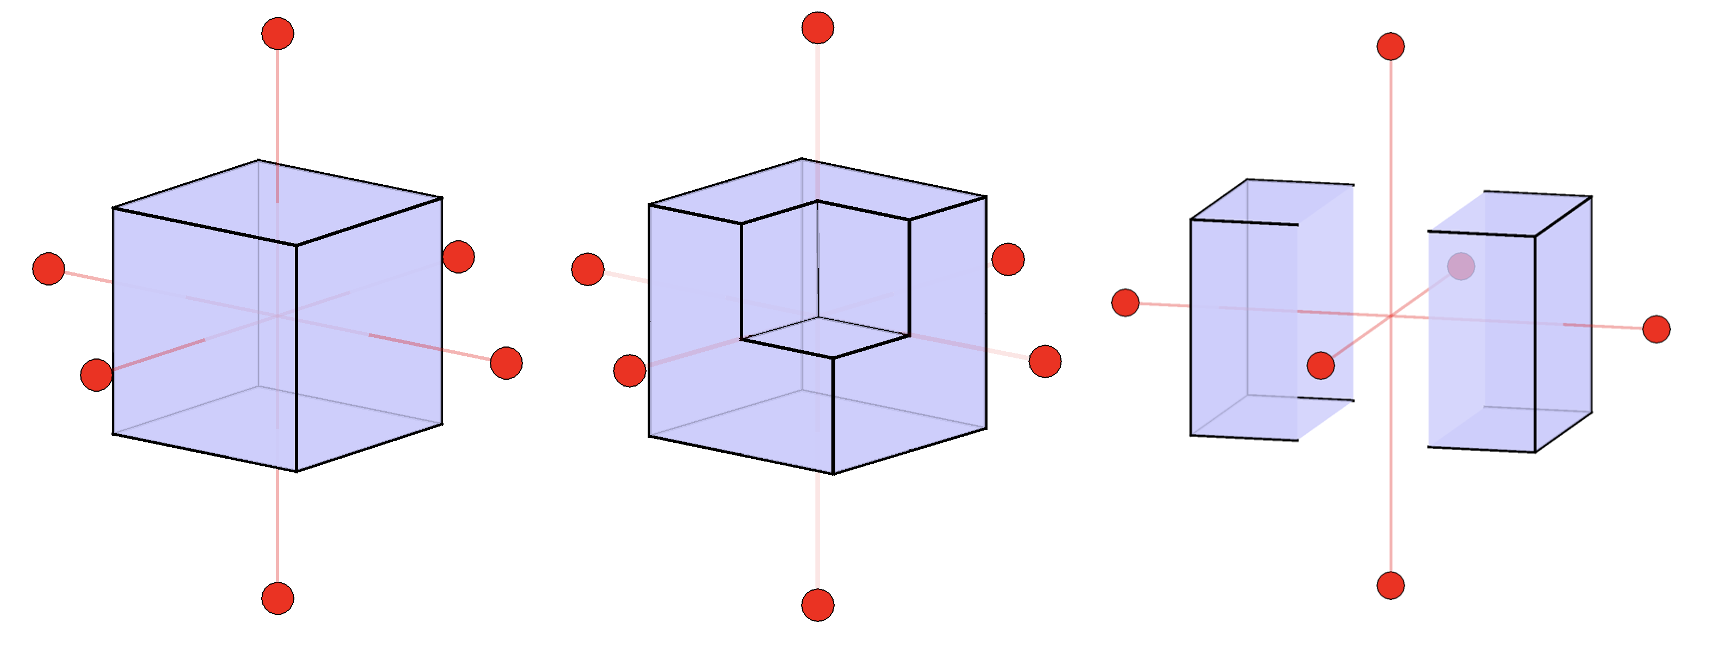
\includegraphics[width=\figmed]{convex_non_open_egis.png}
  \caption{Simplified convex, nonconvex, and open EGI nonuniqueness. Larger circles indicate greater relative areas assigned to a given normal vector.}
  \label{fig:egi_family}
\end{figure}

\subsection{EGI Optimization}

The EGI fulfills two important criteria for the shape inversion problem: it can be estimated directly from the light curve, attitude profile, and material properties, and uniquely represents a convex object \cite{kaasalainen2001}. Further, the EGI can be transformed into a unique convex object and vice versa through the dual transform and Minkowski problem \cite{little1985, minkowski1909}. 

To accomplish the goal of fitting a convex object to a collection of light curve measurements, it is advantageous to define a compact expression for the expected normalized irradiances of a convex object. This is accomplished through the convex reflection matrix $G \in \mathbb{R}^{n \times m}$ with $ij$th entries $G_{ij}$ defined at time $i$ for each facet $j$ is defined using Eq \ref{eq:brdf_def} and Eq \ref{eq:lc_func_normalized} as the normalized received facet irradiance per unit facet area:

\begin{align*} \numberthis \label{eq:reflection_matrix}
  G_{ij} &= \frac{I_{ij}}{I_s a_j} \\
  &= f_r\left(L, O \right) \left(L_j \cdot N_i\right) \left(O_j \cdot N_i\right).
\end{align*}

It must be noted that Eq \ref{eq:reflection_matrix} assumes that the BRDF of the object is uniform across its surface. This is a core assumption of the direct convex inversion scheme in the literature, and a limitation of the method that cannot be easily circumvented. This relationship between the received normalized irradiance and the areas of the object faces reveals the compact form of Eq \ref{eq:lc_func_normalized} for convex objects for any BRDF:

\begin{equation} \label{eq:convex_lc_with_g}
  \hat{I}_{convex} = G \vec{a}.
\end{equation}

Given a light curve, direct shape inversion schemes sample $m$ candidate normal vectors $\hat{n}$ on the unit sphere to fit an EGI to the observed light curve $\hat{I}_\textrm{obs} \in \mathbb{R}^{n \times 1}$ \cite{friedman2020, fan2020thesis}. This is accomplished by solving an optimization problem to distribute the area vector $\vec{a}$ across the sampled normals to minimize the residual between the observed and modeled light curves. In practice, this is a constrained nonnegative least squares (NNLS) problem and can be solved efficiently for large numbers of normal vectors $\hat{n}$ and light curve data points $\hat{I}_\textrm{obs}$:

\begin{equation} \label{eq:area_opt_convex}
  \min_{\vec{a}}{\|\hat{I}_{\textrm{obs}} - G \vec{a}\|_2} \:\:\: \textrm{ subject to } \vec{a}_i \geq 0,
\end{equation}

to yield an optimal set of face areas $\vec{a}_i$. In Eq \ref{eq:area_opt_convex}, the reflection matrix $G$ is computed from the chosen normal vectors $\hat{n}_i$, the uniform BRDF, and the Sun and observer vectors in the body frame of the object. NNLS problems are efficiently solved via Lawson and Hanson's original algorithm \cite{lawson1976}, or the more recent Fast NNLS (FNNLS) algorithm due to Bro and De Jong \cite{bro1996}. It is important to note that the area estimated with Eq \ref{eq:area_opt_convex} is the \textit{albedo-area} due to the reflectivity coefficients in Eq \ref{eq:lc_func_normalized} or \ref{eq:lc_normalized_engine}. If the value of $C_d$ and $C_s$ are uniform with a known ratio $C_d / C_s$, the recovered geometry will be scaled without impacting the face adjacency or relative feature sizes.

The optimization in Eq. \ref{eq:area_opt_convex} produces a coarse approximation of the true EGI as $m$ is finite. Increasing $m$ necessarily improves the quality and sparsity of the estimated EGI, but at the cost of computational resources. The estimation was performed using a synthetic light curve input from $n=500$ Sun and observer vectors uniformly sampled on the sphere in the body frame, producing a full rank $G$ matrix. $m = 500$ candidate normal vectors were sampled using a spherical Fibonacci mapping described by Keinert et al.\ in \cite{keinert2015}. Results are visualized for an icosahedron in the body frame in Figure \ref{fig:initial_egi_sampling}. Reconstructing the object at this stage is difficult due to the quantity of faces present in the estimated EGI. 

\graphicspath{{/Users/liamrobinson/Documents/PyLightCurves/docs/build/html/_images}}
\begin{figure}[!htb]
  \centering
  \includegraphics[width=\figmed]{sphx_glr_egi_figs_aas22_002.png}
  \caption{Initial EGI optimization example for a cube, using 500 candidate normal vectors, the Phong BRDF with $C_d=0.5$, $C_s=0.5$, $n=10$. Relative face area denoted by higher sphere opacity, reference shape shown in grey.}
  \label{fig:initial_egi_sampling}
\end{figure}

\subsection{EGI Observability}

For a given set of candidate normal vectors, the ability to recover a reliable solution from the area optimization problem is known as its observability. As studied by Friedman, the EGI optimization is observable if the Gramian matrix --- $G^T G$ in this case --- is full rank \cite{friedman2020}.

This conclusion follows from an unconstrained least squares estimation of the EGI, and is generally equivalent to the statement that the areas of $n$ normal vectors can be estimated if $m>=n$ measurements are taken with at least one nonzero entry in each column of the reflection matrix $G$. As noted by Cabrera et al.\, the nonnegative constraint placed on the face areas $a_j$ mean that the constrained EGI optimization is often estimatable even when the unconstrained form is unobservable \cite{cabrera2021}. As a result, the unconstrained least squares observability condition is a very conservative lower bound, but is still useful for quantifying the shape information content of the light curve through the rank of $G^T G$. All inversions results presented in this work are performed with observable measurement geometry. 

The EGI observability exposes a new shape ambiguity. If any areas of the EGI are unobservable, the geometry of those portions of the object are entirely unconstrained when considering the light curve alone.

\subsection{EGI Resampling}

A normal vector resampling step is presented in this work to promote a more accurate and sparse EGI. The normal vectors used in Fig \ref{fig:initial_egi_sampling} are generally correct, with each group clustering around a normal vector of the truth geometry. This clustering behavior occurs when none of the candidate normal vectors are sufficiently close to the truth. Resampling in a cone centered on each initial EGI normal vector provides more accurate candidates for EGI estimation. This process mimics a single optimization step with a much larger $m$, where the coarse EGI is used to exclude areas on the sphere with little or no normal area.

Uniformly sampling a cone of half-angle $\phi$ is accomplished by strategically sampling points on the unit sphere. 

\begin{equation} \label{eq:cone_sample_n_pole}
  \hat{n}_{cone} = \begin{bmatrix}
    \sqrt{1-z^2}\cos{\theta} \\
    \sqrt{1-z^2}\sin{\theta} \\
    z \\
  \end{bmatrix}
\end{equation}

In Eq \ref{eq:cone_sample_n_pole} two coordinates are chosen $z \in [\cos{\phi}, 1]$ and $\theta \in [0, 2\pi)$, yielding a point uniformly distributed on a cone of half-angle $\phi$ about the central axis $[0, 0, 1]^T$ \cite{cone_sampling_wolfram}. These points are then rotated using a direction cosine matrix to center the cone on an axis of interest. The axis of rotation for this transformation is the cross product of the original central axis $[0, 0, 1]^T$ with the final axis $\hat{n}_{cone}$ with the rotation angle $\theta$ being the angle between the same two vectors. The principal rotation parameter form of this transformation is given in Eq \ref{eq:cone_sampling_rv} which can be converted into the DCM using Eq \ref{eq:quat2dcm} and \ref{eq:prp2quat}.

\begin{align*} \label{eq:cone_sampling_rv} \numberthis
  \theta &= 2 \cos^{-1}\left( \hat{n}_{cone,z} \right) \\
  \lambda &= \hat{n}_{cone} \times [0, 0, 1]^T
\end{align*}

The number of new candidates sampled per initial solution vector and the cone half-angle should be adjusted on a case-by-case basis depending on the compute power available and light curve data quality. Multiple iterative methods exist for solving nonnegative constrained least squares (NNLS) problems. The classical NNLS algorithm was published by Lawson and Hanson and improved later by Bro and De Jong in their Fast NNLS (FNNLS) approach \cite{lawson1976, bro1996}.

Existing EGI optimization schemes like those of Fan \cite{fan2020thesis}, Friedman \cite{friedman2020}, and Cabrera \cite{cabrera2021} are limited by a single normal vector sampling step, leading to a lack of sparsity in the optimized EGI. High-density normal vector sampling in regions known to contain non-zero area leads to EGI solutions that are generally more sparse and cluster more tightly about true normal vectors. An example of this process is shown in Figure \ref{fig:resampled_egi}.

\begin{figure}[!htb]
  \centering
  \includegraphics[width=\figmed]{sphx_glr_egi_figs_aas22_003.png}
  \caption{Resampled EGI for the cube data using $\phi = \frac{\pi}{20}$, $100$ candidate vectors per resampled cone. Relative face area denoted by higher sphere opacity, reference shape shown in grey.}
  \label{fig:resampled_egi}
\end{figure}

\subsection{EGI Merging}

After resampling and optimizing again with Eq. \ref{eq:area_opt_convex}, the reestimated EGI is merged by computing all groups $\mathcal{G}$ of EGI vectors within an angular offset $\theta_\mathrm{merge}$:

\begin{equation} \label{eq:egi_merge}
  \mathcal{G}_k = \left\{ \vec{E}_i \in \vec{E} \:\| \cos^{-1}\left( \frac{\hat{E}_i \cdot \hat{E}_k}{\|\vec{E}_i \| \| \vec{E}_k \|}\right) < \theta_\mathrm{merge} \right\}.
\end{equation}

In practice, the choice of $\theta_\mathrm{merge}$ is dependent on the user's tolerance for discretization, as merging will approximate smooth geometry by discrete faces with normal vectors offset by $2\theta_\mathrm{merge}$. Groups are merged by summing all group members, yielding a single EGI vector $\vec{E}_m$ without loss of closure. 

\begin{equation} \label{eq:fixing_egi}
  \vec{E}_m = \sum_{\vec{E} \in \mathcal{G}_k}{\vec{E}}
\end{equation}

Merging the resampled EGI shown in Figure \ref{fig:resampled_egi} produces a final sparse EGI fit for object reconstruction, shown in Figure \ref{fig:merged_egi}. 

\begin{figure}[!htb]
  \centering
  \includegraphics[width=\figmed]{sphx_glr_egi_figs_aas22_004.png}
  \caption{Merged EGI for the cube data using $\alpha = \frac{\pi}{10}$. Relative face area denoted by higher sphere opacity, reference shape shown in grey.}
  \label{fig:merged_egi}
\end{figure}

\subsection{Geometry Recovery from the EGI}

At this stage, the resampled and merged EGI encodes a convex approximation of the underlying object with no guarantee of the closure of this EGI. The EGI closure constraint Eq \ref{eq:egi_closure} motivates a simple procedure to correct an invalid EGI by adding the mean closure error to each entry:

\begin{equation} \label{eq:egi_validation}
  \vec{E}_{\textrm{closed}} = \vec{E}_{\textrm{open}} - \sum_{i=1}^m a_i \hat{n}_i .
\end{equation}

The concept of a closure step is not a novel contribution. Fan's method solved an optimization problem to adjust the EGI towards closure \cite{fan2020thesis}. This process is improved with a simpler analytical correction. In practice this process should be performed before each reconstruction to accelerate convergence. Failing to correct non-closed EGIs will cause convergence to a nonzero minimum in the reconstruction objective function as there is no corresponding convex object with the given EGI.

The unique convex object encoded by each closed EGI is reconstructed by solving for the polytope's set of vertices $\mathcal{V}$ and faces $\mathcal{F}$ encoding the adjacency relations between vertices. This is accomplished following the procedure introduced by Little through the dual transformation \cite{little1983}. The dual set $\mathcal{D}$ are vertices in $(A, B, C) \in \mathbb{R}^3$ that satisfy the following plane condition for a point $(x, y, z)$ on each face of the object:

\begin{equation} \label{eq:dual_abc_form}
  Ax + By + Cz + 1 = 0
\end{equation}

If $(x, y, z)$ are chosen to be the closest points in the object's planes to the origin, the dual set $\mathcal{D}$ can be expressed in terms of the EGI and a support vector $\vec{h} \in \mathbb{R}^{\|F\| \times 1}$, where the support vector is the vector of perpendicular distances of each face of the object to the origin. The points of the dual $\mathcal{D}_i \in \mathbb{R}^3$ is expressed in terms of the EGI and the supports as:

\begin{equation} \label{eq:dual_egi_form}
  \mathcal{D}_i = \frac{\vec{E}_i}{ \| \vec{E}_i \| \vec{h}_i}.
\end{equation}

The object's vertices $\vec{v}_{ref}$ are found by solving a linear system of equations for each face on the convex hull of dual set vertices. Triplets of vertices on the resulting faces are used to find a single real vertex by intersecting the three planes defining the dual set vertices.

\begin{equation} \label{eq:vertex_recovery}
  \begin{bmatrix}
    v_{ref,x} \\
    v_{ref,y} \\
    v_{ref,z} \\
  \end{bmatrix} = \begin{bmatrix}
    v_{i,x} & v_{j,x} & v_{k,x} \\
    v_{i,y} & v_{j,y} & v_{k,y} \\
    v_{i,z} & v_{j,z} & v_{k,z}
  \end{bmatrix}^{-1} \begin{bmatrix}
    1 \\ 1 \\ 1
  \end{bmatrix}
\end{equation}

Convex face adjacency information is found by triangulating the convex hull of all reference vertices. The accuracy of the recovered geometry is entirely dependent on the correctness of the support vector $\vec{h}$ used to produce the dual set. Finding the true support vector is the challenge of the final optimization in convex shape inversion.

\subsection{Support Vector Optimization}

This work adopts the same objective function proposed by Little for the support vector optimization as used by Fan \cite{little1983, fan2020thesis}. Little's objective function leverages work of Minkowski, who proved that any closed EGI is a unique representation of a convex object, up to a translation \cite{little1983}. In the literature, these convex shapes in $\mathbb{R}^3$ are known as polytopes. In particular, that unique polytope is merely a scaling and translation from the polytope with volume $1$ that minimizes $\vec{h} \cdot \| \vec{E} \|$ \cite{little1985}. This formulates the support vector optimization problem:

\begin{align*} \numberthis \label{eq:little_problem}
  & \min_{\vec{h}}\left\{ \vec{h} \cdot \| \vec{E} \| \right\} \\
  & \textrm{such that } \frac{1}{3}\left(\vec{h} \cdot \vec{a} \right) = 1
\end{align*} 

Notice that there is a difference between $ \| \vec{E} \| $, the areas of the faces on the desired polytope, and $\vec{a}$, the areas of the polytope recovered by constructing a convex object with the dual transform using Eqs \ref{eq:dual_egi_form} and \ref{eq:vertex_recovery}. This means that a convex object must be fully constructed at each step of the optimization to compute the objective function value. This optimization is highly nonlinear, as adjusting the support of one face may dramatically change both the areas of surrounding faces as well as the volume of the resulting polytope. Due to the convexity of the problem, an initial guess of $\vec{h} = \mathbf{1}$ is sufficient.

Depending on the optimizer, additional function evaluations will be needed to evaluate support gradient as well as the Jacobian of the constraints. Many optimizers struggle with this optimization problem, either due to an inability to meet the constraint or instability that leads to unbounded supports. Little implemented a constrained gradient descent scheme from scratch, showing good results for reconstructing simple objects \cite{little1983}. Gardner solved an equivalent optimization problem using an unspecified solver in MATLAB \cite{gardner2003}. In this work, trust-region methods \cite{conn2000} were found to be robust at solving this optimization.

\section{Direct Nonconvex Shape Inversion}

\subsection{Nonconvex Feature Detection and Location}

Many human-made space objects are, as highlighted in Figure \ref{fig:hst_bennu_shadows}, highly nonconvex. As a result, their shape inversion is plagued by the fact that the Minkowski problem-driven reconstruction methods of Eq \ref{eq:little_problem} cannot recover nonconvex features. Instead of beginning from the ground up, the convex shape guess can be leveraged to detect and locate concavities.

Information about large, unilateral object concavities is obtained during EGI estimation in Eq. \ref{eq:area_opt_convex} by relaxing the EGI closure constraint. This unconstrained form is also generally functional for most convex objects and can be used without loss of detail in the final reconstruction as long as closure correction in Eq. \ref{eq:fixing_egi} is still employed.

The mean axis of prominent concave features is determined by measuring the divergence of the optimized EGI from a closed object with the magnitude of the closure error $\vec{e}_{EGI}$.

\begin{equation} \label{eq:closure_error}
  \vec{e}_{EGI} = -\sum_{i=1}^{m} a_i \hat{n}_i.
\end{equation}

The EGI closure error vector in Eq \ref{eq:closure_error} represents the missing area on each body axis that could be added to close the object. The addition of the minus sign transforms the vector from expressing the presence of excess area to the absence of missing area. The closure error will be negligible if there are no concavities present. The closure error may also be negligible if there is no self-shadowing present over the sampled attitude profile, therefore the closure error merely quantifies the self-shadowing present in the measurements, not whether there may be self-shadowing in other orientations.

Under the strong assumption that the concavities present are major and unilateral, this EGI error vector points along the mean axis of the concavity. This is because self-shadowing in that region causes brightness measurements to be smaller than expected for the true area present, leading to an optimized EGI that attributes less area to that section of the object. As a result, summing the EGI entries produces a vector that points away from the concavity, requiring the negation seen in Eq \ref{eq:closure_error} to point towards it.

\subsection{Concavity Creation}

Given the direction of a supposed concavity in the body frame of the object, the next challenge is introducing that concavity. This work approximates unknown concave features as valleys with sharp floors, adopting the interior angle $\psi$ between the valley walls as the measure of the feature depth. An interior angle of $\psi=180^\circ$ implies no concavity, whereas $\psi \rightarrow 0^\circ$ will push the concavity through the object entirely.

The proposed process for creating an accurate concavity in the reconstructed convex guess proceeds in four major steps. The model is first subdivided to add more faces and vertices. Subdivided vertices are then classified by their proximity to the EGI error vector, indicating whether their positions should be updated. Boundary vertices are identified, and vertex positions are updated based on an internal angle. The light curve error of that nonconvex guess is computed, and the internal angle is iterated until a suitable minimum error case is identified.

\subsection{Model Subdivision}

Subdividing the initial convex object guess is essential for retaining object detail during concavity creation. A combination of linear subdivision, Loop subdivision, and remeshing algorithms are used to accomplish this. Linear subdivision is advantageous when object faces are equally sized and boundary edges must be maintained. Loop subdivision is preferable when there are numerous vertices so that subdivisions do not drastically diverge from the initial boundary surface. Loop subdivision softens sharp edges as it relies on B-splines to interpolate new vertex positions \cite{loop1987}. The specific type and resolution of subdivision used depends on the level of detail the user needs to maintain in the introduced concavity, although linear subdivision followed by Loop subdivision is a useful baseline. Varying combinations of subdivision are shown in Figure \ref{fig:subd_grid} to illustrate the available configurations.

\graphicspath{{/Users/liamrobinson/Documents/msthesis/static_images/aas_2022_figs}}
\begin{figure}[!htb]
  \centering
  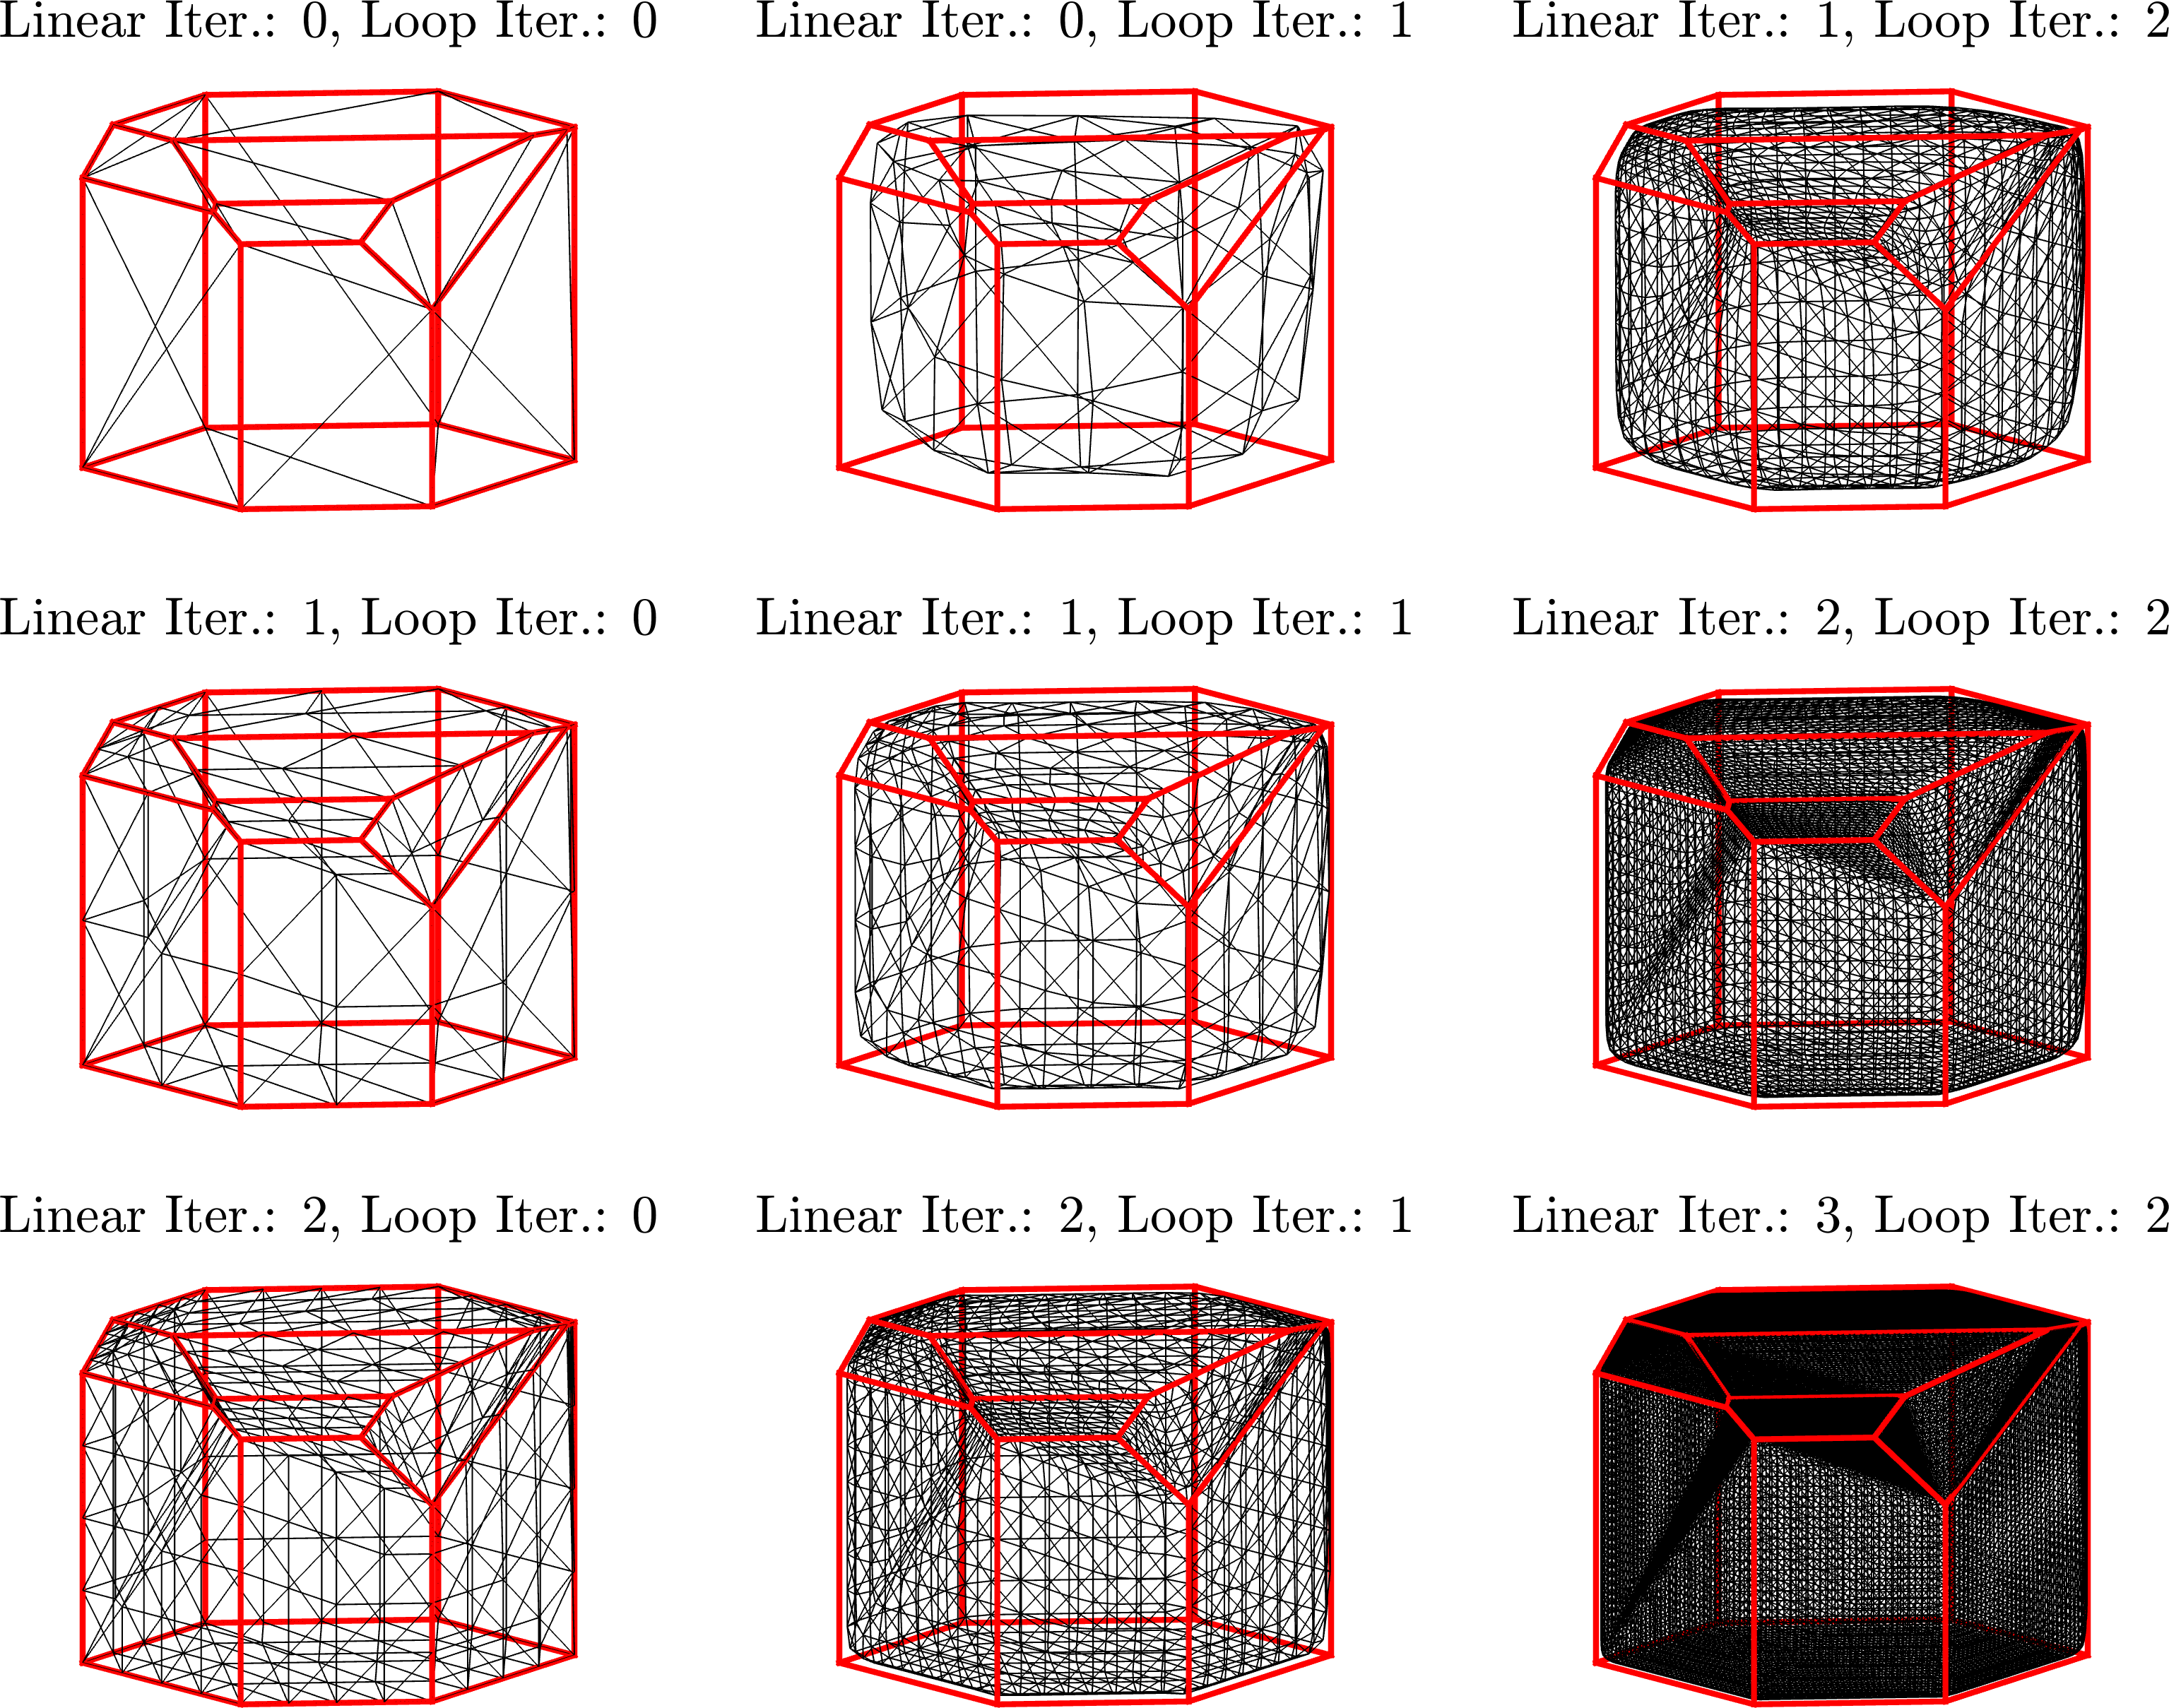
\includegraphics[width=350px]{subd_grid.png}
  \caption{Subdivided object (black) with reference (red) with various levels of subdivision}
  \label{fig:subd_grid}
\end{figure}

\subsection{Vertex Classification}

When introducing a concavity, it is important to classify which vertices are part of the concave feature --- and therefore need to be updated --- and which vertices should remain unaffected. This is accomplished by measuring the angle from each face normal to the EGI error vector, where faces with normal vectors within an angle of $\pi/2 - \varepsilon$ to the error vector must be updated, where $\varepsilon$ is a bias angle that controls the conservativeness of the classification. Choosing $\varepsilon=0$ selects all faces above the horizon from the EGI error vector and may lead to concavities that encompass too much of the object. Generally, $\varepsilon \in [0.3, 0.7]$ rad is effective. In reality, all face normals and areas are impacted by the presence of the concavity in the area optimization Eq. \ref{eq:area_opt_convex} and EGI correction step Eq \ref{eq:egi_validation}. This bound tends to produce visually accurate concavities. Faces requiring an update are termed \textit{free} faces, with all others termed \textit{root} faces. Explicitly, each face $F_i$ is classified $C(F_i)$ via:

\begin{equation} \label{eq:root_free}
  C(F_i) = \begin{cases} 
    0 & \cos^{-1}\left( \hat{n}_i \cdot \hat{e}_{EGI} \right) \geq \frac{\pi}{2} - \varepsilon \\
    1 & \cos^{-1}\left( \hat{n}_i \cdot \hat{e}_{EGI} \right) < \frac{\pi}{2} - \varepsilon \\
  \end{cases}.
\end{equation}

In Eq \ref{eq:root_free}, $C(F_i) = 0$ implies a root face, with $C(F_i) = 1$ implying a free face. Vertices on free faces are further classified as being \textit{root-adjacent} or \textit{free}. Root-adjacent vertices are part of at least one root face, whereas free vertices belong to only free faces. The classification of each vertex $\vec{v}_i$ via $C(\vec{v}_i)$ is expressed via:

\begin{equation} \label{eq:root_free_verts}
  C(\vec{v}_i) = \begin{cases}
    0 & \sum_{j \in \mathcal{N}(\vec{v}_i)}{C(F_j)} = 0 \\
    1 & \sum_{j \in \mathcal{N}(\vec{v}_i)}{C(F_j)} > 0 \\    
  \end{cases} \: \: \forall i \in \left\{ i \mid C(F_i) = 1 \right\}.
\end{equation}

In Eq \ref{eq:root_free_verts}, $\mathcal{N}(\vec{v}_i)$ is the set of face indices including $\vec{v}_i$ as a vertex, yielding $C(\vec{v}_i) = 0$ to imply a free vertex, and $C(\vec{v}_i) = 1$ to imply a root-adjacent face. Classifying vertices in this way results in a border of root-adjacent vertices around the interior free vertices, visualized in Figure \ref{fig:root_and_free}.

\begin{figure}[!htb]
  \centering
  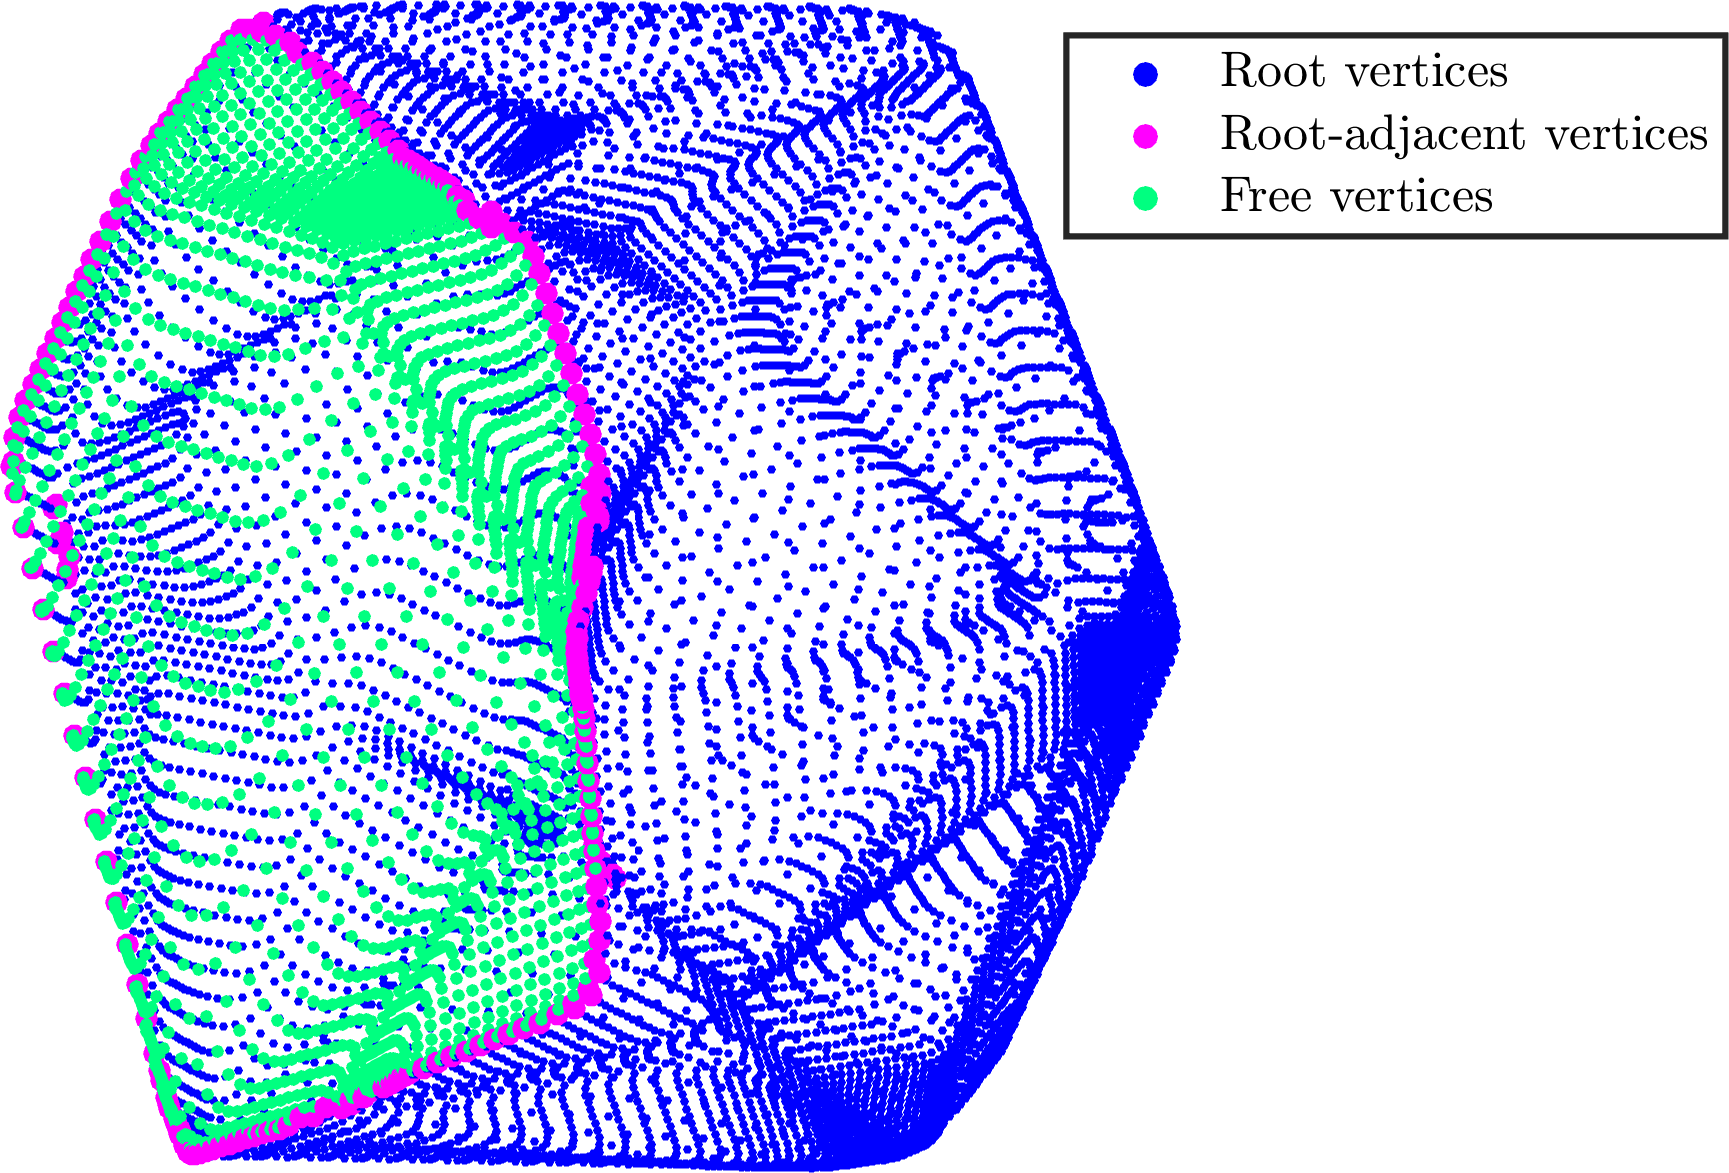
\includegraphics[width=250px]{rootadj_and_free_verts_try2.png}
  \caption{Root-adjacent and free vertices}
  \label{fig:root_and_free}
\end{figure}

\subsection{Vertex Displacement}

Given the estimated internal angle $\psi_{est}$ and the error vector $\hat{e}_{EGI}$, each $i$th free vertex is displaced to introduce a geometrically accurate concavity by moving each a distance $d_i$ in the direction of $-\hat{e}_{EGI}$:

\begin{equation} \label{eq:flip_depth}
  d_i = p_i \sqrt{\csc^2 \frac{\psi_{est}}{2} - 1},
\end{equation}

where $p_i$ is the distance from each $i$th free vertex to the nearest root-adjacent vertex.

\subsection{Internal Angle Iteration}

Prior work by the author indicated an analytical relationship between this interior angle and the norm of the EGI error vector, summarized in Figure \ref{fig:misleading_egi_error} \cite{robinson2022}.

\begin{figure}[!htb]
  \centering
  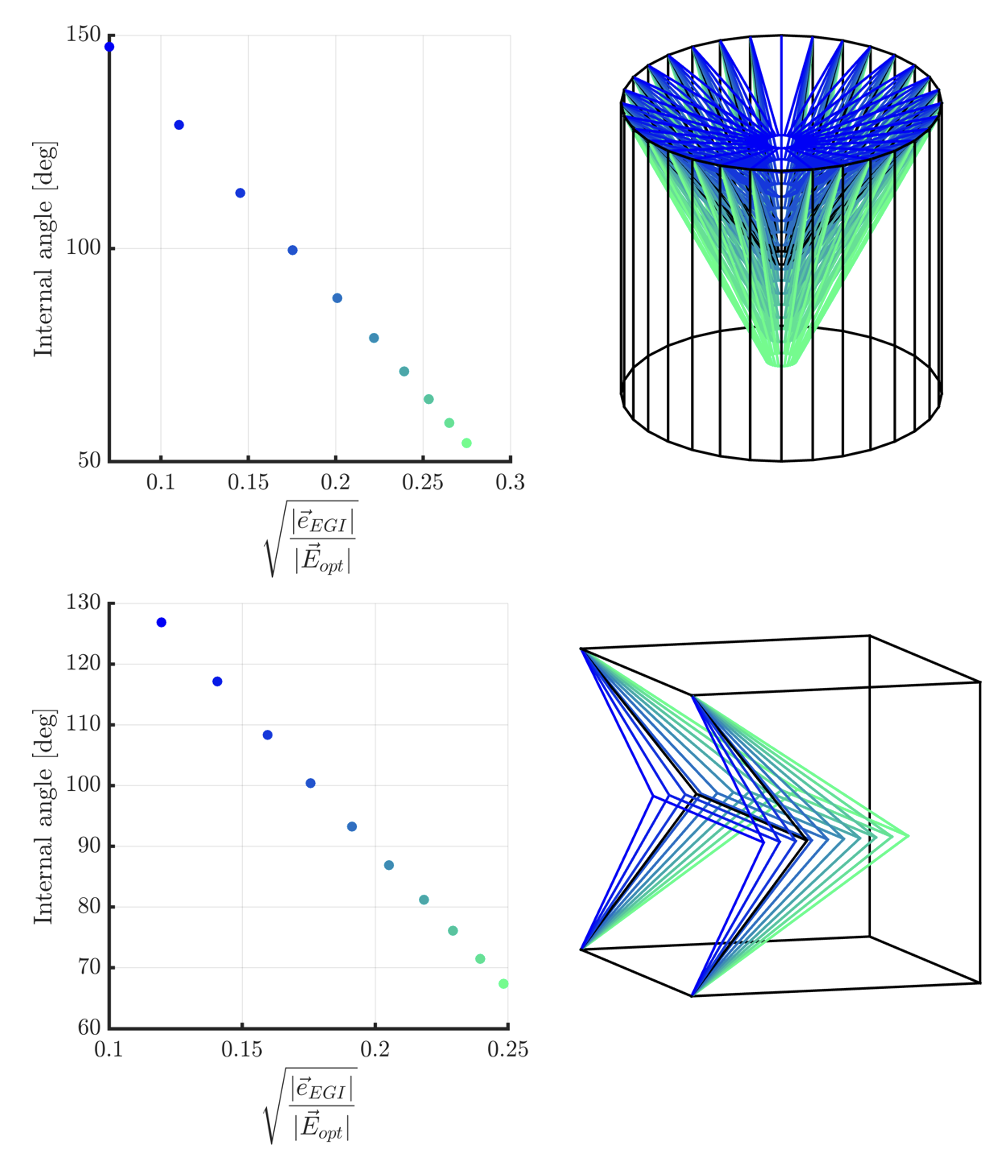
\includegraphics[width=\figsmall]{error_mag_study/combined_error_mag.png}
  \caption{EGI error relationship to internal angle for the collapsed cylinder and collapsed house from \cite{robinson2022}}
  \label{fig:misleading_egi_error}
\end{figure}

The objects in Figure \ref{fig:misleading_egi_error} were illuminated with a simple Lambertian BRDF and the brightness measurements used to optimize the EGI were produced by randomly sampled Sun and observer vectors. Once specular effects and non-random observation conditions are accounted for, the linear relationship between $\psi$ and $\sqrt{\frac{\|\vec{e}_{EGI}\|}{\|\vec{E}\|}}$ no longer exists. In short, the optimal concavity angle $\psi_{opt}$ is sought such that:

\begin{equation} \label{eq:psi_opt}
  \psi_{opt} = \min_{\psi} \left( \| \hat{I} - \hat{I}(\psi) \| \right),
\end{equation}

where $\hat{I}$ is the observed normalized light curve and $\hat{I}(\psi)$ is the light curve resulting with Eq \ref{eq:lc_normalized_engine} using a nonconvex mesh with a concavity of angle $\psi$ introduced. In practice, a line search is sufficient to find the interior angle that minimizes the light curve error of the reconstructed object, summarized in Algorithm \ref{alg:concavity_iter}.

\begin{algorithm}
  \caption{Concavity sizing algorithm}\label{alg:concavity_iter}
  \begin{algorithmic}
    \State $f_{cvx},v_{cvx}$ \Comment{Faces and vertices of the convex guess}
    \State $f_{subd}, \:v_{subd} \gets \mathrm{Subdivide}(f_{cvx},v_{cvx})$ \Comment{Subdivided convex guess}
    \State $\psi = 180^\circ$ \Comment{Initial guess, no concavity}
    \State $i = 0$ \Comment{Iteration number}
    \While {$i < i_{max}$}
      \State $f_{disp}, \:v_{disp} = \mathrm{DisplaceVertices}(f_{subd},v_{subd})$
      \State $\hat{I}_{i} = \mathrm{LightCurve}(f_{disp}, \:v_{disp})$
      \State $e_i = \| \hat{I} - \hat{I}_{i} \|$
      \State{$\psi \gets \psi + \Delta \psi$}
      \State{$i \gets i + 1$}
    \EndWhile

    $\psi_{opt} = \min_i{e_i}$
  \end{algorithmic}
\end{algorithm}

\section{Shape Inversion With Noisy Measurements}

When the light curve measurements are subject to environmental noise, the shape inversion result --- convex or nonconvex --- may vary significantly from the noiseless shape estimate. Fan addressed this problem most recently with a multiple hypothesis scheme \cite{fan2020thesis}. Given a number of noisy light curves, Fan produced a convex shape estimate from each and ranked each by its error when simulated against a new set of observations \cite{fan2020thesis}. Fan and Frueh later adapted this scheme with a sequential Monte Carlo method, which began identically by producing a collection of convex guesses from samples of the same noisy light curve \cite{fan20201}. The error in each guess was measured against a new noisy light curve, enabling a weighted merge of the estimated EGIs, which was then perturbed to produce a new set of estimated shapes \cite{fan2021}. Throughout these methods, Fan assumed that the noise on the light curve was Gaussian and of constant magnitude, although it was noted that the real character of the noise is dependent on both the geometry of the observation and the magnitude of the signal itself \cite{fan2020thesis}. 

This work presents a method for multiple hypothesis shape inversion that builds on Fan's work by relaxing the constant, Gaussian noise assumption and is agnostic to the convexity of the candidate objects. This new method also uses an face-dependent estimate of the uncertainty in each candidate shape's geometry, yielding final object estimates that take only the most accurate features from each candidate object.

\subsection{Weighted Shape Interpolation}

To develop this multiple hypothesis inversion procedure that works for both convex and nonconvex shape candidates, it is useful to be able to take a weighted average of an arbitrary set of triangle meshes. Given candidate object meshes $M_i$ with scalars $w_i$, this weighted average process should be of the form:

\begin{equation}
  M_{\mathrm{interp}} = \sum_{i}{w_i M_i}.
\end{equation}

The algorithm presented in this work for weighted mesh averaging depends on signed distance fields (SDFs). The SDF implicitly represents a shape by associating each point $\vctr{x} \in \mathbb{R}^3$ with the distance to the closest point on the surface of the object \cite{baerentzen2002}. As a result, the gradient of the SDF points directly away from the closest piece of the object's geometry. For a given SDF $f(\vctr{x})$, the surface of the object $\mathcal{S}_\mathrm{obj}$ is given by all points $\vctr{x}$ that yield $f(\vctr{x}) = 0$:

\begin{equation} \label{eq:sdf_zero_level_set}
  \mathcal{S}_\mathrm{obj} = \left\{ \vctr{x} \in \mathbb{R}^3 \mid f(\vctr{x}) = 0 \right\}.
\end{equation}

Computing the SDF of a triangulated mesh breaks down into computing distances from the points, line segments, and planes making up the mesh to the queried point \cite{baerentzen2002}. A slice of the SDF of a test model is displayed in Figure \ref{fig:sdf_slice}.

\graphicspath{{/Users/liamrobinson/Documents/PyLightCurves/docs/build/html/_images}}
\begin{figure}[!htb]
  \centering
  \includegraphics[width=\figmed]{sphx_glr_sfds_001_2_00x.png}
  \caption{SDF slice of the Stanford bunny model}
  \label{fig:sdf_slice}
\end{figure}

Interpolating three-dimensional meshes using signed distance fields is not a novel concept proposed by this work. Cohen-Or et al.\ used distance fields with anchor points to find warping functions between two geometries \cite{cohen_or1998}. A simple interpolation strategy between two shapes can be accomplished through a weighted average of the respective SDFs. If both objects are weighted at $50\%$, the weighted sum of their SDFs produces a surface that lies halfway in between the two original shapes, measured perpendicular to the input objects' surfaces. This interpolated zero level set surface can be extracted through any three-dimensional isocontouring algorithm such as marching cubes \cite{lorensen1987} or flying edges \cite{schroeder2015}. For example, interpolating between a torus and an icosahedron using this method yields Figure \ref{fig:interpolating_torus_ico}. 

\begin{figure}[!htb]
  \centering
  \includegraphics[width=\figmed]{sphx_glr_shape_interpolation_001.png}
  \caption{SDF interpolation between a torus and an icosahedron}
  \label{fig:interpolating_torus_ico}
\end{figure}

The proposed algorithm for shape interpolation for SDF interpolation of two shapes $M_1, M_2$ with convex weights $w_1, w_2$ is:

\begin{algorithm}
  \caption{SDF interpolation}\label{alg:sdf_interp}
  \begin{algorithmic}
  \Require $w_1 + w_2 = 1$
  \State $\mathrm{SDF}_{\textrm{interp}} \gets w_1 \cdot \mathrm{SDF}_{M_1} + w_2 \cdot \mathrm{SDF}_{M_2}$
  \State $M_{\textrm{interp}} = \mathrm{Isocontour}(\mathrm{SDF}_{\textrm{interp}}, 0)$.
  \end{algorithmic}
\end{algorithm}

Algorithm \ref{alg:sdf_interp} can operate on arbitrary convex or nonconvex meshes, making it well suited to interpolating between light curve inversion results.

The procedure in Algorithm \ref{alg:sdf_interp} can be further generalized by allowing the weights $w_i$ to be functions of the location in $\mathbb{R}^3$ of each SDF grid point:

\begin{equation}
  \mathrm{SDF}_{\mathrm{interp}}(x, y, z) = w_1(x, y, z) \cdot \mathrm{SDF}_{M_1}(x, y, z) + w_2 \cdot \mathrm{SDF}_{M_2}(x, y, z).
\end{equation}

To discourage degenerate behavior, it is necessary to enforce $w_i(x,y,z) > 0 \forall (x,y,z) \in \mathbb{R}^3$.

\subsection{Shape Estimate Uncertainty}

When merging multiple inaccurate shape guesses it is advantageous to measure the uncertainty in each candidate shape and use that uncertainty as a weighting to bias the merging process. The formulation used in this work relies on two face-wise uncertainty terms. First, a face should have high uncertainty if very little light would have reflected off that face to contribute to the light curve. Second, that face should also have high uncertainty if its reflected light has highly contaminated by background noise. As a result, the only faces of an estimated shape with low uncertainty should be those that reflect a large \textit{quantity} of light, increasing the observability of that face, while being uncontaminated by the background to yield a high \textit{quality} signal. These uncertainty terms are computed by first scaling the columns of the reflection matrix defined in Eq \ref{eq:reflection_matrix} by the area of each respective face $a_j$:

\begin{equation} \label{eq:h_matrix}
  H_{ij} = a_j G_{ij}.
\end{equation}

The resulting matrix $H$ has the same dimensions as $G$, but has entries $H_{ij}$ representing the normalized irradiance expected from face $j$ and time $i$. The total normalized irradiance over all timesteps for each face is given by:

\begin{equation} \label{eq:total_norm_irrad}
  \hat{I}_{j} = \sum_{i}{H_{ij}}.
\end{equation}

Computing $\hat{I}_{j}$ is useful as it represents the total quantity of signal expected from face $j$ across the light curve. Using this value, the data quantity weighting is:

\begin{equation} \label{eq:unc_quantity}
  u_{quant,j} = 1 - \frac{\hat{I}_{j} - \min_{j}{\hat{I}_{j}}}{\max_{j}{\hat{I}_{j}} - \min_{j}{\hat{I}_{j}}}.
\end{equation}

Interpreting Eq \ref{eq:unc_quantity}, the face with the most influence on the overall light curve is assigned a data quantity uncertainty of $u_{quant,j} = 0$ while the face with the least influence is assigned $u_{quant,j} = 1$. This meets the first requirement for the uncertainty measure sought; a large quantity of data should produce an accurate final shape estimate. This is further motivated by investigating the statistical nature of the light curve signal. As the object signal is Poisson distributed, the signal itself is well-modeled as a Poisson distribution independently sampled at each timestep. Since the sum of two Poisson distributions with mean and variance $\lambda_1$ and $\lambda_2$ is also Poisson with parameter $\lambda_3 = \lambda_1 + \lambda_2$, the total variance of the sum of the light curve $\lambda_\mathrm{lc}$ is:

\begin{equation}
  \lambda_\mathrm{lc} = \sum_{i} C_{obj,meas,i},
\end{equation}

implying that as the sum of the signal magnitudes grow linearly, their standard deviation $\sqrt{\lambda_\mathrm{lc}}$ grows sublinearly. As a result, a higher quantity of available data for a face will will always exponentially lower the SNR. That said, a high quantity of available data does not necessarily mean that the data has a high SNR. Estimating the SNR in the measured counts is certainly possible, especially if the observing station is well characterized, but is a strong assumption for an unknown ground station. It would be preferable to estimate the variance of the measured signal through the convex shape guess itself. As the NNLS optimization of the EGI is guaranteed to produce the convex shape that best matches the measured irradiances, the convex guess is a good estimator for the mean of the received signal so long as the noise on the measurements is zero mean. As a result, the variance of the light curve error:

\begin{equation}
  \mathrm{Var}\left(\delta \hat{I}\right) = \mathrm{Var}\left(Ga - \hat{I}_{meas}\right)
\end{equation}

generally matches the true signal and noise variance. This means that scaling the expected normalized irradiance $H_{ij}$ by the absolute value of the light curve error yields a quantity that is proportional to the number of false counts above or below the true mean attributed to a certain face:

\begin{equation}
  \delta \hat{I}_{tot,j} = a_j \sum_{i}{\left( G_{ij} a_j - \hat{I}_{meas,i} \right) H_{ij}},
\end{equation}

yielding a weighting for the data quality attributed to each face of the convex guess:

\begin{equation} \label{eq:u_qual}
  u_{qual,j} = \frac{\delta \hat{I}_{tot,j} - \min_{j}{\delta \hat{I}_{tot,j}}}{\max_{j}{\delta \hat{I}_{tot,j}} - \min_{j}{\delta \hat{I}_{tot,j}}}.
\end{equation}

Eq \ref{eq:u_qual} can be interpreted in terms of the statistical properties of the light curve just like Eq \ref{eq:unc_quantity}. Under the assumption that the EGI optimized by NNLS produces a good estimator for the mean of the measured light curve, higher environmental noise will produce a larger residual $\delta \hat{I}_{tot,j}$ at a given signal magnitude. As a result, the term $u_{quant,j}$ can be seen as accounting for the variance of the object signal --- which becomes less impactful as the object signal grows --- while the term $u_{qual,j}$ acocunts for the variance of the environmental noise --- which acts to degrade the light curve signal regardless of the object signal magnitude.

These two uncertainty weightings are combined at each face for a global uncertainty estimate:

\begin{equation} \label{eq:u_total}
  u_{j} = \frac{u_{qual,j}}{2} + \frac{u_{quant,j}}{2}.
\end{equation}

Eq \ref{eq:u_total} is formulated such that a face is only assigned a low uncertainty if it has both high data quality and quality. A face with the lowest quality and quantity will be assigned $u_{j} = 1$ while simply having bad quality or quantity alone yields $u_j = 0.5$, thereby discounting low quantities of high quality data as well high quantities of low quality data. Figure \ref{fig:face_uncertainties} displays the quality, quantity, and overall uncertainty weighting for the faces of a convex shape guess.

\begin{figure}
  \centering
  \begin{subfigure}[b]{0.3\textwidth}
      \centering
      \includegraphics[width=\textwidth]{sphx_glr_face_uncertainty_005.png}
      \label{fig:quant_weights}
  \end{subfigure}
  \hfill
  \begin{subfigure}[b]{0.3\textwidth}
      \centering
      \includegraphics[width=\textwidth]{sphx_glr_face_uncertainty_006.png}
      \label{fig:qual_weights}
  \end{subfigure}
  \hfill
  \begin{subfigure}[b]{0.3\textwidth}
      \centering
      \includegraphics[width=\textwidth]{sphx_glr_face_uncertainty_007.png}
      \label{fig:qual_overall}
  \end{subfigure}
  \caption{Quantity (left), quality (middle), and overall face uncertainty (right) weights}
  \label{fig:face_uncertainties}
\end{figure}

Figure \ref{fig:face_uncertainties} conveys that $u_{qual}$ and $u_{quant}$ convey independent information about each face depending on the measured light curve and its noise --- higher data quantity does not necessarily imply higher quality.

\subsection{Spherical Nearest Neighbor Weights} \label{sec:nearest_sphere}

One final challenge remains: translating the uncertainties of the faces of an object to a weighting function that can be applied throughout $\mathbb{R}^3$ to weight the SDF. Simply projecting points onto the unit sphere and performing nearest-neighbor interpolation accomplishes this task well. For a set of reference points $\vctr{r}_{i}$ each with a weight $w_i$, the weight index $i_q$ of query point $\vctr{r}_q \in \mathbb{R}^3$ is the solution to:

\begin{equation}
  i_{q} = \min_{i}\left( \| \vctr{r}_q - \vctr{r}_i \| \right).
\end{equation}

In practice, this is solved with a Balltree, a spatial search data structure designed to efficiently find nearest neighbors in $n$-dimensional space bounded by the $n-1$-dimensional sphere \cite{omohundro1989}. The result of this nearest neighbor interpolation for a number of query points is shown in Figure \ref{fig:ball_tree_nn_interp}.

\begin{figure}[!htb]
  \centering
  \includegraphics[width=\figmed]{sphx_glr_spherical_voronoi_interp_001.png}
  \caption{Nearest neighbor interpolation between reference points (red) with uniformly distributed weights on $[0,1]$.}
  \label{fig:ball_tree_nn_interp}
\end{figure}

The final spherical weighting $w(\vctr{r}_q)$ applied to each object at a given query point location $\vctr{r}_q \in \mathbb{R}^3$ is the certainty of the nearest face $1-u_j(\vctr{r}_q)$ scaled by the light curve error of that object:

\begin{equation} \label{eq:merge_weighting}
  w(\vctr{r}_q) = \left( 1-u_j(\vctr{r}_q) \right) \left( \hat{I}_{meas} - \hat{I}_\mathrm{obj} \right),
\end{equation}

where $\hat{I}_{meas}$ is the measured normalized light curve produced by Eq \ref{eq:ihat_meas} and $\hat{I}_\mathrm{obj}$ is the normalized light curve produced by the shape estimate under the same observation conditions.

\subsection{Full Noisy Inversion Procedure} \label{sec:mh_inversion}

Given $n$ noisy light curves from an object of unknown shape, the procedure determining a single best estimate of the object's true shape has three stages. 

\begin{enumerate}
  \item Convex shape guesses are computed for each noisy light curve.
  \item Each shape is checked for potential nonconvex features by introducing singular concavities in the direction of the EGI error vector following Algorithm \ref{alg:concavity_iter}. Each nonconvex guess along with the convex guess is simulated in the same observation conditions to compute an error with respect to the original light curve. The guess --- convex or nonconvex --- with the lowest error is selected moving forward.
  \item Now with $n$ convex or nonconvex shape estimates, one for each original light curve, the uncertainty in each face of each object is computed with Eq \ref{eq:u_total}.
  \item Given these uncertainties, each object is assigned a spherical weighting function $w_i(x, y, z)$ via Eq \ref{eq:merge_weighting}.
  \item The objects are merged together via their weights using the SDF procedure outlined by Algorithm \ref{alg:sdf_interp}, yielding a final shape estimate.
\end{enumerate}

